\section{Internship at IBM}\
This bachelor's thesis covers the concrete specification of the internship project, the company in which the internship took place, the research needed to complete the project and the practical implementation. The internship project was provided by IBM in Brussels as part of the \acrfull{gbs} division.
\subsection{IBM}
IBM, which is an acronym for International Business Machines, is a leading and innovative corporate entity active the field of information technology. The focus has shifted away from hardware-only solutions to a vast array of solutions due to the development in IT and electronics \cite{IBMa}. The predominant solutions that IBM offers are:
\begin{enumerate}
\item Blockchain;
\item Cloud Computing;
\item Artificial Intelligence;
\item Watson IoT;
\item Analytics;
\item Java;
\item Security;
\item Open Source;
\item Global Technology Services;
\end{enumerate}
IBM has seen an increase in revenue from their Cloud and Analytics solutions in 2019 due to continuous improvements in their data centers and ever-expanding expert employees \cite{Condon2019}.
\subsection{Internship Team}
Below, the team of interns is displayed.
\begin{figure}[h!]
\centering
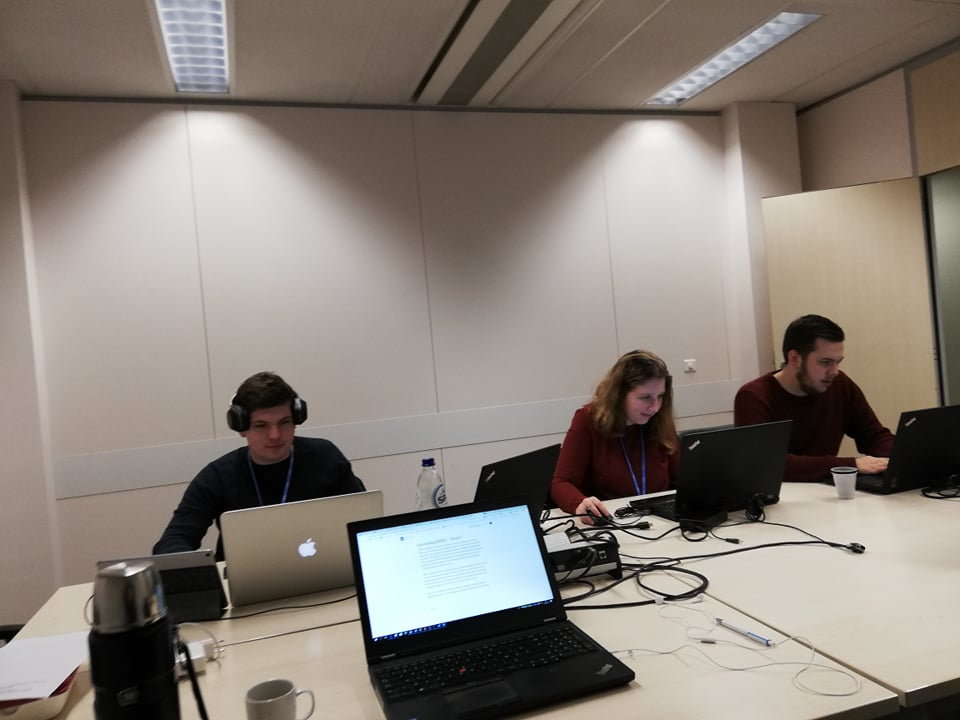
\includegraphics[scale=0.4]{interns}
\caption{The team of interns}
\label{fig:toa}
\end{figure}

